% !TEX TS-program = pdflatex
% !TEX encoding = UTF-8 Unicode

% This is a simple template for a LaTeX document using the "article" class.
% See "book", "report", "letter" for other types of document.

\documentclass[11pt]{article} % use larger type; default would be 10pt

\usepackage[utf8]{inputenc} % set input encoding (not needed with XeLaTeX)

%%% Examples of Article customizations
% These packages are optional, depending whether you want the features they provide.
% See the LaTeX Companion or other references for full information.

%%% PAGE DIMENSIONS
\usepackage{geometry} % to change the page dimensions
\geometry{a4paper} % or letterpaper (US) or a5paper or....
% \geometry{margin=2in} % for example, change the margins to 2 inches all round
% \geometry{landscape} % set up the page for landscape
%   read geometry.pdf for detailed page layout information

\usepackage{graphicx} % support the \includegraphics command and options

% \usepackage[parfill]{parskip} % Activate to begin paragraphs with an empty line rather than an indent

%%% PACKAGES
\usepackage{booktabs} % for much better looking tables
\usepackage{array} % for better arrays (eg matrices) in maths
\usepackage{paralist} % very flexible & customisable lists (eg. enumerate/itemize, etc.)
\usepackage{verbatim} % adds environment for commenting out blocks of text & for better verbatim
\usepackage{subfig} % make it possible to include more than one captioned figure/table in a single float
% These packages are all incorporated in the memoir class to one degree or another...

%%% HEADERS & FOOTERS
\usepackage{fancyhdr} % This should be set AFTER setting up the page geometry
\pagestyle{fancy} % options: empty , plain , fancy
\renewcommand{\headrulewidth}{0pt} % customise the layout...
\lhead{}\chead{}\rhead{}
\lfoot{}\cfoot{\thepage}\rfoot{}

%%% SECTION TITLE APPEARANCE
\usepackage{sectsty}
\allsectionsfont{\sffamily\mdseries\upshape} % (See the fntguide.pdf for font help)
% (This matches ConTeXt defaults)

%%% ToC (table of contents) APPEARANCE
\usepackage[nottoc,notlof,notlot]{tocbibind} % Put the bibliography in the ToC
\usepackage[titles,subfigure]{tocloft} % Alter the style of the Table of Contents
\renewcommand{\cftsecfont}{\rmfamily\mdseries\upshape}
\renewcommand{\cftsecpagefont}{\rmfamily\mdseries\upshape} % No bold!

%%% END Article customizations

%%% The "real" document content comes below...

\title{STU33009 Week 9 Assignment}
\author{Efeosa Louis Eguavoen -  17324649}
%\date{} % Activate to display a given date or no date (if empty),
         % otherwise the current date is printed 

\begin{document}
\maketitle

\section{Question 1}
(a)
\begin{verbatim}
def gradient_descent():
    function = lambda x: (x**2) -1
    xvals = []
    yvals = []
    for i in range(-10,10,1):
        xvals.append(i)
    yvals = list(map(function,xvals))
   # plt.plot(xvals,yvals)
    #plt.show()
   # print(xvals,'\n',yvals)

    startX = 2.5
    learningRate = float(input('Enter Learning Rate: '))
    precision = 0.000001
    prev_size = 1
    max_iters = 1000
    cur_Iter = 0
    func = lambda x: 2*x

    while prev_size > precision and cur_Iter < max_iters:
        prev_x = startX
        inter = float(func(prev_x))
        startX = startX - learningRate * float(func(prev_x))
        prev_size = abs(startX-prev_x)
        cur_Iter = cur_Iter+1
        print("Iteration", cur_Iter, "\nX value is", startX)
    print("The local minimum occurs at", startX)
\end{verbatim}

(b)
\newline
For a= 1 we get the following plot:
\begin{center}
	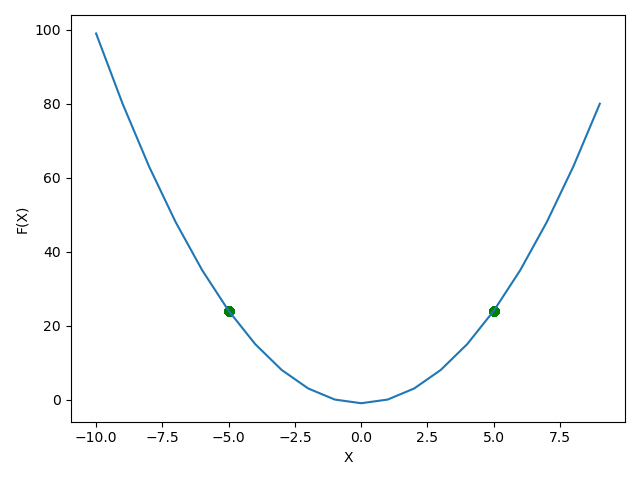
\includegraphics[scale = 0.5]{a2.png}
\end{center}
As we can see on the graph, F(x) swithces between -5 and 5 when the learning parameter is 1 as we essentially keep shooting past the minnimum each iteration through the loop.
\newline
\newline
For a = 0.1 we get this plot:
\begin{center}
	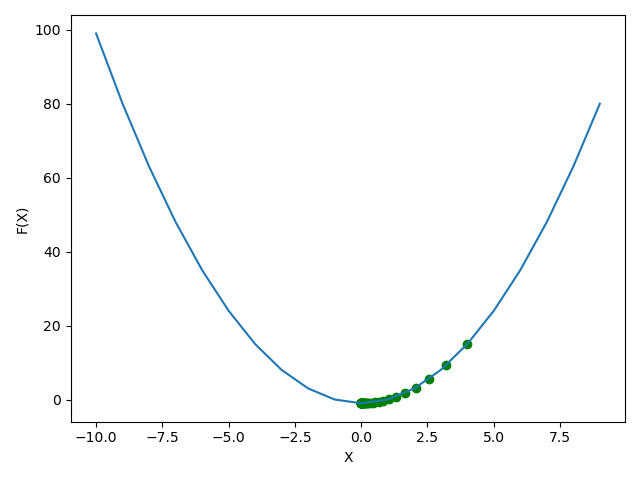
\includegraphics[scale = 0.5]{a02.png}
\end{center}
From this graph, we can see the f(x) approaching our minimum each time we iterate through the loop. Our learning parameter enables us to approach the minnmum at a good pace and enables the loop to exit in much fewer iterations than when compared to other 0.01 for instance.
\newline
\newline
For a = 0.01 we get this plot:
\begin{center}
	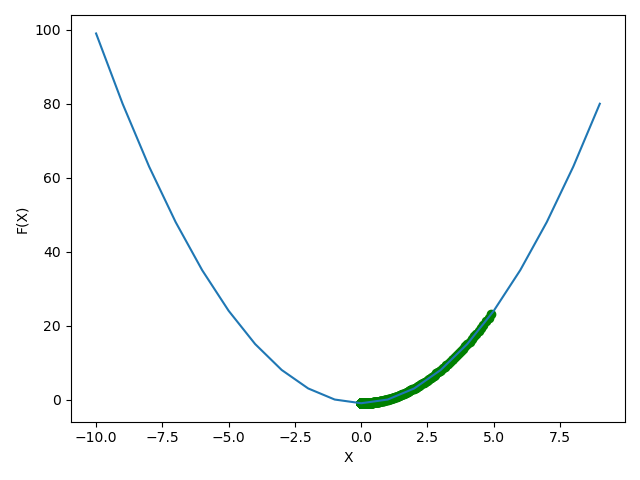
\includegraphics[scale = 0.5]{a002.png}
\end{center}
Again, we see f(x) approaching the minnimum but requires way more iterations of the loop to exit and progress is much slower than when we were using 0.1 as out learning parameter. We do eventually reach the minnimum but the number of iterations is way more than when we used 0.1.
\newline
\newline
(c)
\begin{verbatim}
def gradient_descentRandom():
    function = lambda x: (x ** 2) - 1
    xvals = []
    yvals = []
    for i in range(-10, 10, 1):
        xvals.append(i)
    yvals = list(map(function, xvals))
    plt.plot(xvals, yvals)
    print(xvals, '\n', yvals)

    startX = 5
    precision = 0.000001
    prev_size = 1
    max_iters = 1000
    cur_Iter = 0
    derX = []
    while cur_Iter < max_iters:
        randomX = random.uniform(startX-1,startX+1)
        if function(randomX) < function(startX):
            startX = randomX
            derX.append(startX)
        cur_Iter = cur_Iter + 1
    derY = list(map(function, derX))
    plt.scatter(derX, derY, c='g')
    plt.show()
    print("The local minimum occurs at", startX)
\end{verbatim}
Example output:
\begin{center}
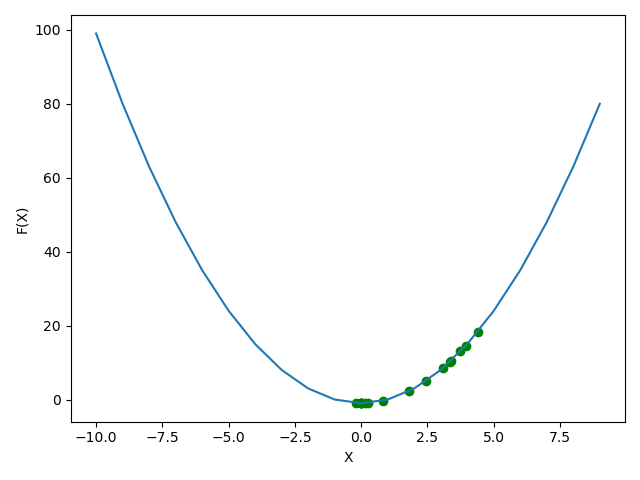
\includegraphics[scale = 0.5]{r2.png}
\end{center}
We can see it's random as the gap between points isn't consistently getting smaller as a number is chosen at random each time in the vincinity of X.
\newline
\newline
(d)
\newline
The random approach can work when given enough iterations(in my code I gave it 1000 iterations) to approach the minnimum but it's a lot slower also there's no guarantee it will reach the actual minimum in the given amount of loops as it's totally random. Also there's no way of making the loop exit early reliably as there's no guarantee of the next point possibly increasing the value of x. The gradient descent approach works better as we can definitely approach the mininmum over a number of iterations but we need to be careful to choose a learning value that won't overshoot the minimum. Also it's a lot faster as we can make it exit early if given a precision level we're looking for.

\section{Question 2}
(a) 
\newline
To classify the hotel reviews, we can define a model 
\[y = h\theta(x) \]
with it's parameters being 
\[\theta0,\theta1...\]
Each of the values of theta equal to a value in the feature vector for that review.
\[h\theta(x) = sign(\theta1X1,\theta2X2... \theta nXn\]
\newline
(b)
\newline
We need to assume that the dependant variable is binary i.e that what output we get will either be positive or negative mapping each to 0 and 1 respectively.
\newline
(c)
\newline
?
\end{document}
